\documentclass[conference]{IEEEtran}
\usepackage{cite}
\usepackage{graphicx}
\usepackage{url}
\usepackage{booktabs}
\usepackage{array}
\usepackage{listings}
\usepackage{xcolor}
\usepackage{tikz}
\usepackage{adjustbox}
\usetikzlibrary{arrows.meta,positioning,fit,calc,shapes.geometric}
\def\UrlBreaks{\do\/\do-\do\_\do\.\do\?\do\&\do\=}

\definecolor{codebg}{RGB}{248,250,252}
\definecolor{codeframe}{RGB}{203,213,225}
\definecolor{codestring}{RGB}{3,105,161}
\definecolor{codekey}{RGB}{126,34,206}
\definecolor{codecomment}{RGB}{71,85,105}
\definecolor{codekw}{RGB}{185,28,28}

\lstdefinelanguage{json}{
  basicstyle=\ttfamily\scriptsize,
  showstringspaces=false,
  breaklines=true,
  morestring=[b]",
  stringstyle=\color{codestring},
  literate=
   *{0}{{{\color{codekey}0}}}{1}
    {1}{{{\color{codekey}1}}}{1}
    {2}{{{\color{codekey}2}}}{1}
    {3}{{{\color{codekey}3}}}{1}
    {4}{{{\color{codekey}4}}}{1}
    {5}{{{\color{codekey}5}}}{1}
    {6}{{{\color{codekey}6}}}{1}
    {7}{{{\color{codekey}7}}}{1}
    {8}{{{\color{codekey}8}}}{1}
    {9}{{{\color{codekey}9}}}{1}
    {:}{{{\color{black}:}}}{1}
    {,}{{{\color{black},}}}{1}
    {\{}{{{\color{black}\{}}}{1}
    {\}}{{{\color{black}\}}}}{1}
    {[}{{{\color{black}[}}}{1}
    {]}{{{\color{black}]}}}{1},
}

\lstdefinelanguage{rust}{
  morekeywords={struct,enum,pub,Option,String,bool,i64,u64,u32,JsonValue},
  sensitive=true,
  morecomment=[l]{//},
  morestring=[b]",
}

\lstdefinestyle{api}{
  backgroundcolor=\color{codebg},
  frame=single,
  rulecolor=\color{codeframe},
  basicstyle=\ttfamily\scriptsize,
  keywordstyle=\color{codekw}\bfseries,
  commentstyle=\color{codecomment},
  stringstyle=\color{codestring},
  columns=fullflexible,
  keepspaces=true,
  showstringspaces=false,
  breaklines=true,
  breakatwhitespace=false,
  tabsize=2,
  xleftmargin=0.6em,
  xrightmargin=0.6em,
  captionpos=t,
  abovecaptionskip=0.8em,
  belowcaptionskip=1.25em,
  aboveskip=1.1em,
  belowskip=2.2em
}
\lstset{
  captionpos=t,
  abovecaptionskip=0.8em,
  belowcaptionskip=1.25em,
  aboveskip=1.1em,
  belowskip=2.2em
}
\makeatletter
\newlength{\jeryulistingcaptiongap}
\setlength{\jeryulistingcaptiongap}{0.9\baselineskip}
\let\jeryu@orig@lst@makecaption\lst@makecaption
\def\lst@makecaption#1#2{%
  \jeryu@orig@lst@makecaption{#1}{#2}%
  \par\nobreak\vskip\jeryulistingcaptiongap\nobreak
}
\makeatother

\title{JeRyu: A Proof-Carrying, Agent-First Git Control Plane}

\author{\IEEEauthorblockN{JeRyu Project}
\IEEEauthorblockA{Draft for V3.01\\
Agent-first GitLab control plane, VTI, evidence, and merge-gate architecture}}

\begin{document}
\maketitle

\begin{abstract}
Modern software agents can edit code faster than conventional review, CI, and release systems can safely absorb. GitHub Copilot cloud agent can research, plan, edit branches, run tests, and create pull requests, but public documentation describes important constraints: one branch at a time, one pull request per task, and GitHub-hosted repositories only \cite{github-copilot-cloud-agent}. GitLab Duo Agent Platform brings agentic automation into GitLab contexts, including issues, merge requests, pipelines, planning, and security signals \cite{gitlab-duo-ga,gitlab-duo-platform,gitlab-duo-workflow}. Open-source agents such as OpenHands, SWE-agent, and Aider improve code authoring and task execution, but generally remain outside the Git/CI authority boundary \cite{openhands-paper,sweagent-paper,aider-repo}. JeRyu proposes a different layer: an agent-first delivery control plane that treats agent intent, validation plans, CI execution, runner trust, cache use, failure evidence, merge gates, and release gates as one proof loop. Its VTI subsystem maps changes to validation with conservative fallback, while the V3.01 plan upgrades this into proof receipts, selector-miss learning, typed capabilities, admission enforcement, and a TUI operations console.
\end{abstract}

\begin{IEEEkeywords}
software engineering agents, CI/CD, GitLab, smart test selection, validation, evidence, merge gates, agent safety
\end{IEEEkeywords}

\section{Introduction}
Agent-first development changes the bottleneck. Code generation is no longer the only scarce resource; trustworthy validation becomes scarce. Public coding-agent workflows now let developers delegate issue implementation, branch creation, test execution, and pull request creation \cite{github-copilot-cloud-agent,github-copilot-howto}. GitLab has similarly moved toward lifecycle-wide agentic automation across project context, CI/CD, security findings, and planning surfaces \cite{gitlab-duo-ga,gitlab-duo-platform,gitlab-duo-docs}. Open-source agents have also raised expectations for terminal use, repository exploration, and autonomous repair \cite{openhands-paper,sweagent-paper,aider-repo}. These systems are important, but they leave a gap for teams that need local-first, policy-controlled, proof-scoped autonomy over runners, sandboxes, cache, merge gates, release gates, and evidence retention.

JeRyu is designed around that gap. Instead of making an agent imitate a human in a browser, it gives agents typed control surfaces: capability intents, validation planning, job traces, failure capsules, merge readiness, release status, cache verdicts, runner pools, and a TUI that exposes the same state to human supervisors. The long-term claim is not that agents should receive unrestricted control. It is that agents should receive bounded authority and produce durable evidence for every action that matters.

This paper describes the V3.01 direction for JeRyu. It uses the repository itself as the artifact under study: a Rust workspace with a \texttt{jeryu} binary, proof-scoped support crates, GitLab-oriented orchestration, VTI smart test selection, a capability API, a Ratatui console, and deterministic paper screenshots. The contribution is a control-plane pattern for agent-first development:

\begin{enumerate}
\item a proof loop that connects intent, policy, validation, evidence, and merge or release decisions;
\item a VTI model that saves test time only when it can explain what was skipped and why;
\item a capability model that makes action availability canonical across API, CLI, and TUI surfaces;
\item a screenshot-capable operations console that makes agent behavior reviewable; and
\item a V3.01 roadmap for hardening admission, state, merge gates, dynamic CI, and selector-miss learning.
\end{enumerate}

\section{Public Capability Baseline}
GitHub Copilot cloud agent can work in the background, research a repository, create implementation plans, fix bugs, improve tests, update documentation, resolve merge conflicts, and operate in a GitHub Actions-powered environment \cite{github-copilot-cloud-agent}. Public limitations matter for control-plane design: the documented cloud agent operates on one branch at a time, opens one pull request per task, and is scoped to GitHub-hosted repositories \cite{github-copilot-cloud-agent}. GitHub exposes integrations through issues, pull requests, agents panels, IDEs, GitHub CLI, Slack, Teams, Linear, Jira, Azure Boards, and MCP-compatible tools \cite{github-copilot-howto,mcp-spec}. These are strong product surfaces, but they are not a local GitLab runner authority layer.

GitLab Duo Agent Platform, generally available in GitLab 18.8, positions agents across the software lifecycle with organization context and guardrails \cite{gitlab-duo-ga,gitlab-18-8}. GitLab describes Agentic Chat and Duo Workflow use cases for code analysis, CI/CD troubleshooting, planning, security analysis, issues, merge requests, and pipelines \cite{gitlab-duo-platform,gitlab-duo-workflow,gitlab-agent-platform-intro,gitlab-duo-workflow-blog}. GitLab's public material also emphasizes human governance, enterprise context, and platform integration \cite{gitlab-duo-handbook}. JeRyu is complementary but narrower: it is not a general assistant; it is a GitLab-compatible control plane built to decide what an agent may do, what proof it must provide, and which local resources it may touch.

OpenHands is an open platform for software development agents that can write code, use terminals, and browse the web \cite{openhands-paper,openhands-site,openhands-repo}. SWE-agent introduced an agent-computer interface for automated software engineering \cite{sweagent-paper}. Aider provides terminal-centered pair programming \cite{aider-repo}. Codex-style local and cloud agents emphasize task execution across terminal, IDE, web, and pull request workflows \cite{openai-codex,github-openai-codex,openai-codex-system-card}. These tools are valuable authoring engines, yet authoring is not the same as production authority. The control-plane question is: what validates the agent, records its authority, constrains its side effects, and prevents unsafe merge or release?

\section{Empirical Pressure}
The need for proof-carrying delivery follows from observed agent failure modes. Studies and datasets around software engineering agents show both promise and fragility: benchmark tasks can be solved, but real pull requests still require human modification, review, and rejection handling \cite{swebench,swebench-verified,aidev-dataset,agent-pr-modifications}. Work on agentic pull requests reports failed and unmerged agent contributions as a recurring operational pattern \cite{failed-agentic-prs,agent-prs-unmerged}. Traceability research argues that software agents need stronger links among task, change, evidence, and outcome \cite{software-agents-traceability}. This is consistent with decades of automated repair work: a generated patch is not a proof of correctness \cite{repair-survey}.

Continuous integration already encodes a social contract: code is acceptable only after running the appropriate validation under a known configuration \cite{continuous-integration}. Regression test selection and prioritization literature adds nuance: selective testing can reduce cost, but unsafe selection can miss failures \cite{regression-test-selection-survey,safe-regression-test-selection,test-prioritization}. Agent-first systems stress this contract because they can produce more branches, more experiments, and more merge requests than humans can manually supervise. JeRyu therefore treats validation choice itself as an auditable artifact.

\section{Why Git Must Change}
Agent-first and ``vibe coding'' workflows shift the economic center of software delivery. When code generation becomes cheap, validation, review, provenance, and release authority become the scarce resources. The correct response is not to run fewer tests; it is to run the right tests, preserve proof for skipped tests, and make validation scale with the number of agent hypotheses. Coverage pressure will rise because agents can generate more code paths, more branches, and more plausible-but-wrong fixes than conventional human review can absorb.

Legacy Git forges were built around human-paced pull requests, human-scoped credentials, and CI as a background reaction to commits. That model can be extended with assistants, but extension is not the same as redesign. Agent-first development needs Git to understand task identity, capability grants, validation receipts, cache trust, runner isolation, proof-carrying merge decisions, and cleanup of speculative work. A Rust control plane is a pragmatic fit for this layer: it can sit close to Git, CI, filesystems, sockets, runners, and local policy while remaining fast enough for high-churn agent loops.

The paper's central claim is therefore structural. Future developers will not keep pace with AI by waiting for hosted  platforms to retrofit every proof boundary. They need an open-source, agent-first substrate where validation and authority are first-class product concepts rather than conventions around a pull request. JeRyu keeps GitLab compatibility where useful, but places the agent proof loop under local, inspectable control.

\section{Architecture}
JeRyu is a Rust workspace with a \texttt{jeryu} binary and proof-scoped support crates. The control plane includes CLI and TUI surfaces, a Unix-socket capability API, GitLab webhook ingestion, Postgres-primary state with SQLite fallback, runner pools, custom executor hooks, VTI, release gates, and proof-routing utilities. It consumes GitLab concepts such as pipelines, runners, custom executors, protected branches, and CI artifacts \cite{gitlab-ci-docs,gitlab-runners-docs,gitlab-custom-executor,gitlab-protected-branches}. It also interoperates conceptually with GitHub-style workflow constraints and branch protection semantics \cite{github-actions-docs,github-branch-protection}.

\begin{figure}[t]
\centering
\fbox{\begin{minipage}{0.94\linewidth}
\small
\begin{tabular}{@{}p{0.22\linewidth}p{0.68\linewidth}@{}}
\textbf{Intent} & agent action, actor, task, grant, idempotency key\\
\textbf{Policy} & path scope, branch scope, risk tier, trust tier, budget\\
\textbf{Plan} & VTI lanes, selected tests, skipped tests, fallback reason\\
\textbf{Execute} & runner pool, sandbox, cache namespace, CI pipeline\\
\textbf{Evidence} & logs, failure capsule, test receipt, cache verdict\\
\textbf{Decide} & merge gate, release gate, cleanup, durable memory
\end{tabular}
\end{minipage}}
\caption{JeRyu proof loop. Agents do not jump directly from patch to merge; they move through intent, policy, validation, evidence, and decision records.}
\label{fig:proof-loop}
\end{figure}

The architecture differs from a bot wrapper. A bot wrapper receives an issue and emits a branch. JeRyu owns the delivery loop around that branch. It can select a runner pool, inspect job state, retrieve failure capsules, reason about cache taint, schedule validation, and expose blockers. Postgres gives concurrent local agents a durable coordination layer, while SQLite remains the low-friction embedded fallback for single-node development and tests \cite{postgresql,sqlite}. Tokio and Axum support asynchronous API and webhook execution \cite{tokio,axum}. Bollard gives Docker control for runner and container state \cite{bollard}. Cargo-nextest, cargo-deny, RustSec, SLSA, in-toto, and Sigstore represent the surrounding proof and supply-chain ecosystem that JeRyu is designed to coordinate with rather than replace \cite{rust-cargo-nextest,cargo-deny,rustsec,slsa,in-toto,sigstore}.

\section{Proof-Scoped Workspace}
V3.01 treats repository structure as a proof-routing surface. The workspace contains support crates for witness graphs, validation routing, architectural exception review, runtime witness macros, and ARC/VRC benchmarking. These tools are intentionally local: they reduce the time an agent spends rediscovering ownership and validation rules. \texttt{cargo-witness} indexes public API signatures. \texttt{cargo-vrc} maps changed files to validation rings. \texttt{cargo-aer} audits structural exceptions. \texttt{witness-rt} emits structured repair packets when runtime expectations fail. \texttt{arc-bench} evaluates design tradeoffs.

This matters because an agent often needs two kinds of knowledge. The first is semantic knowledge about code. The second is procedural knowledge about how to prove a change. Public assistants focus heavily on the former. JeRyu makes the latter explicit. A change under \texttt{src/secrets.rs} is not merely a Rust edit; it is a security-relevant proof lane. A change under \texttt{src/test\_intel/} is not merely a module edit; it can affect selector correctness and should widen validation. This repository-level proof routing complements CI systems rather than duplicating them \cite{gitlab-ci-docs,github-actions-docs}.

\section{VTI: Validation Test Intelligence}
VTI is the core latency reducer. The current internal planner maps changed paths to subsystems, applies global invalidators, identifies docs-only changes, selects unit and integration tests, and falls back to full validation when paths are unmapped or confidence is low. External repositories can provide \texttt{.jeryu/testmap.toml}. V3.01 makes the conservative boundary sharper: unknown files force full validation; recursive subsystem patterns cover nested modules; selector misses become scoped evidence; and each skipped test must have a reason that a merge gate can inspect.

Selective validation is valuable only when the skipped work is explained. Classical regression test selection and prioritization show that reduction must be balanced against fault-detection risk \cite{regression-test-selection-survey,safe-regression-test-selection,test-prioritization}. JeRyu therefore represents VTI as a proof generator, not an optimization flag. A VTI plan should say: these files changed; these subsystems are affected; these tests were selected; these tests were skipped; this skip is justified by path ownership, dependency information, and historical evidence; this unknown path caused full fallback.

\begin{table}[t]
\caption{VTI 3.0.1 Validation Outcomes}
\centering
\begin{tabular}{lll}
\toprule
Outcome & Meaning & Merge Semantics\\
\midrule
passed & executed and passed & evidence-positive\\
failed & executed and failed & blocker\\
skipped\_by\_vti & skipped with receipt & evidence-qualified\\
docs\_only & docs allowlist only & low-risk receipt\\
full\_fallback & widened to full & conservative\\
unsafe\_to\_skip & no skip proof & must execute\\
\bottomrule
\end{tabular}
\end{table}

The V3.01 code change moves this direction: unknown file types no longer collapse to docs-only behavior, nested TUI, gateway, and test-intelligence paths now match recursive subsystem patterns, internal plans can emit stable VTI receipts, and the default merge gate treats a missing receipt as a blocker. Remaining work is to persist receipts as first-class state, connect selector-miss records to oracle runs, and bind receipts to live GitLab job evidence. This distinction is essential. A skipped test with a receipt is a qualified claim. A missing test without a receipt is a hole.

\section{Capability and Admission Model}
The current capability API exposes useful intents: \texttt{RunTests}, \texttt{FetchCapsule}, \texttt{ProposePatch}, \texttt{RacePatches}, \texttt{RequestMerge}, \texttt{ExplainBlockers}, \texttt{GetSystemSnapshot}, \texttt{ListAllowedActions}, and \texttt{PlanValidation}. V3.01 adds an agent action envelope with request id, actor, nonce, expiry, optional budget, optional grant proof, and framed JSON transport while preserving  \texttt{AgentIntent} clients. The action registry remains canonical so API, CLI, and TUI do not drift. That is a small implementation change with a large governance consequence: an agent asking what it can do receives the same truth the human console uses.

The target authority model is an intent ledger. An agent requests an action with actor, task, grant, request, and idempotency identifiers. Policy evaluates scope, path rules, branch rules, TTL, risk tier, and budget. The ledger records allow, deny, or escalate before side effects occur. Evidence and cleanup records are attached afterward. This model aligns with the traceability requirement for agent contributions \cite{software-agents-traceability} and with supply-chain systems that separate declaration, execution, and attestation \cite{slsa,in-toto,sigstore}.

Admission control is the server-side counterpart. A pre-receive hook should not merely log suspicious input; it should reject policy violations with structured reasons. Examples include unscoped agent branches, forbidden paths, missing task IDs, unsigned privileged operations, stale base SHAs, or validation receipts that do not match the pushed commit. GitLab protected branch controls provide one perimeter \cite{gitlab-protected-branches}; JeRyu adds agent-aware intent checks inside that perimeter.

\section{Proof-Carrying Merge Gates}
Autonomous merge requires stronger evidence than ``some tests passed.'' V3.01 introduces a shared merge gate used by CLI, TUI, capability API, and webhooks. The gate checks MR identity, exact head SHA, latest pipeline, required jobs, pending jobs, VTI plan confidence, selector misses, cache taints, security/release lanes, branch protection, approvals, conflicts, and stale branch state. Its output is a durable merge proof. A merge is allowed because evidence verifies, not because the agent is trusted.

\begin{table}[t]
\caption{Merge Gate Inputs}
\centering
\begin{tabular}{ll}
\toprule
Input & Required Property\\
\midrule
MR identity & project, IID, source, target, head SHA\\
Pipeline & latest for head SHA, terminal, required jobs passed\\
VTI & selected lanes, fallback status, skip receipts\\
Risk & security/release lanes, trust tier, approvals\\
Cache & no tainted artifacts in proof path\\
Branch & protected target, no conflict, no stale base\\
Evidence & capsules, logs, validation receipts retained\\
\bottomrule
\end{tabular}
\end{table}

The important design choice is that merge decisions are not embedded in one endpoint. A CLI command, TUI action, webhook reconciler, and capability request should call the same gate. Otherwise the system accumulates hidden bypasses. This is especially relevant for agents that can race patches or propose multiple branches. A patch-race feature is useful only if losing branches are cleaned up, winning branches still pass the same gate, and the race result does not become a shortcut around required validation.

\section{Runner, Cache, and Sandbox Boundaries}
Agent-first development increases load on runners and caches. JeRyu therefore treats execution context as part of proof. A trusted branch, an untrusted MR, a release job, and a supply-chain detonation lane should not share the same assumptions. GitLab Runner and custom executor documentation define the execution substrate \cite{gitlab-runners-docs,gitlab-custom-executor}; JeRyu adds trust tiers, BuildKit namespace separation, taint tracking, honeypot detection, and cache promotion rules.

The cache problem is subtle. Smart caching makes CI faster, but unsafe cache reuse can smuggle state across trust boundaries. JeRyu models cache decisions using trust tier, taint, and epoch. A cache hit is not merely a performance event; it is a statement that the artifact is acceptable for this build unit, namespace, and epoch. This aligns with broader supply-chain verification systems that treat artifacts, provenance, and signatures as first-class data \cite{slsa,in-toto,sigstore,rustsec}. Sandbox mechanisms such as gVisor, Firecracker, and Bubblewrap illustrate the isolation vocabulary available for untrusted work \cite{gvisor,firecracker,bubblewrap}.

\section{Agent Workflows}
The intended V3.01 workflow starts with an explicit task. An agent receives a task description and requests capability grants. The control plane creates or verifies a branch, associates it with actor and task identity, and records an intent. The agent may then propose a patch, ask for validation, fetch failure capsules, race alternative hypotheses, or request a merge decision. Each operation is scoped by the same registry and policy layer, so the system can answer what was allowed, what was denied, and why.

A repair loop illustrates the difference from a generic coding assistant. The agent asks for a failing job trace. JeRyu returns a capsule that includes project, job, pipeline, stage, log tail, suspected owner area, and suggested validation lanes. The agent patches the owner area and asks VTI for a plan. VTI selects tests or widens to full validation. The runner executes with the appropriate trust and cache namespace. The merge gate then checks the exact head SHA against the evidence. At no point does the system rely on the agent's verbal claim that it ran tests.

Patch racing is the aggressive version of the same model. Multiple hypothesis branches can be launched in parallel, but every branch needs identity, cleanup policy, and evidence boundaries. The winner is not the fastest branch; it is the branch whose evidence satisfies the gate. Losers should be closed, caches should remain scoped, and the audit ledger should retain enough context to explain the decision. This is where an agent-first GitLab fork can exceed ordinary assistant integration: speed comes from orchestration, not from bypassing proof.

\begin{table}[t]
\caption{Agent Workflow State Machine}
\centering
\begin{tabular}{lll}
\toprule
State & Agent Action & Control-Plane Proof\\
\midrule
planned & request grant & task, actor, scope\\
patched & propose diff & branch, base SHA, paths\\
validated & run VTI plan & jobs, receipts, capsules\\
blocked & explain blockers & failing proof nodes\\
mergeable & request merge & gate decision\\
closed & cleanup & branch/cache records\\
\bottomrule
\end{tabular}
\end{table}

\section{Threat Model}
JeRyu assumes agents are useful but not intrinsically trusted. A capable agent may hallucinate validation, choose an unsafe shortcut, overfit a patch to a narrow test, leak a secret through logs, or unknowingly reuse tainted artifacts. A malicious or compromised agent may try to push to protected paths, create a branch that looks human-owned, replay old validation evidence, or exploit cache state. The defense is not one gate; it is layered evidence.

The first layer is identity and intent. Every privileged action needs actor, task, and idempotency context. The second layer is policy. Path scope, branch rules, risk tier, and grant TTL determine whether an action can proceed. The third layer is execution isolation. Runner pools, sandbox mechanisms, and cache namespaces reduce cross-contamination. The fourth layer is validation. VTI can reduce work only when it emits receipts; otherwise it must fall back. The fifth layer is final decision. Merge and release gates verify current head state, required jobs, approvals, taints, and blockers.

This model deliberately separates productivity from authority. An agent may be excellent at producing patches and still be untrusted for merge. A cache may be effective and still be unusable across trust tiers. A test plan may be fast and still be insufficient for a security-relevant path. V3.01's central hardening target is to make those distinctions concrete in code rather than relying on convention.

\section{TUI and Screenshots}
The TUI is a Ratatui operations surface, not a decorative dashboard \cite{ratatui}. It contains Mission, Release, Jobs, Agents, Tests, Pools, Cache, Evidence, and Secrets tabs. The V3.01 TUI upgrade applies the strongest review theme from the upgrade notes: the console should continuously answer what happened, why it matters, what proof exists, and what the safest next action is. The default Mission view now opens as an action cockpit with a Top Signal, Attention Queue, Proof Stack, next actions, metric tiles, and compact activity graphics. The Agents view now acts as an Agent Cockpit with phase, progress, branch/SHA, grants, timeline, and action guidance. The command palette previews risk, grant requirements, side effects, dry-run availability, and disabled reasons from the canonical action registry.

To support publication and review, V3.01 uses two capture modes:
\begin{itemize}
\item \textbf{PTY render}: runs the TUI inside a real pseudo-terminal, parses the screen state, and renders the grid with a pinned font and palette.
\item \textbf{Deterministic render}: renders Ratatui \texttt{TestBackend} buffers for stable fixture diffs.
\end{itemize}

\begin{lstlisting}[basicstyle=\ttfamily\footnotesize]
./scripts/capture-tui-screenshots.sh
just tui-screenshot-smoke
jeryu tui --capture --tab jobs \
  --output paper/assets/jeryu-tui-jobs-flow.png
\end{lstlisting}

The publication pipeline uses \texttt{jeryu tui --screenshot} inside a real PTY and captures the terminal screen before alternate-screen cleanup. A dedicated \texttt{tui-capture} utility parses the terminal byte stream with a VT parser, validates that the selected font supports box drawing and block glyphs, and renders PNGs with fixed geometry, DejaVu Sans Mono, a lifted dark background, and brightened colors. This avoids browser, SVG, ANSI-to-image, and window-manager font fallback artifacts. The deterministic path remains useful for CI reproducibility. In both modes, screenshots are evidence artifacts backed by demo state snapshots.

\begin{figure}[t]
\centering
\includegraphics[width=\linewidth]{assets/jeryu-tui-jobs-flow.png}
\caption{TUI Jobs/Flow capture showing pipeline flow, live jobs, logs, and events.}
\label{fig:tui-flow}
\end{figure}

\begin{figure}[t]
\centering
\includegraphics[width=\linewidth]{assets/jeryu-tui-tests-vti.png}
\caption{TUI Tests/VTI capture showing selected validation, recent test intelligence, and history context.}
\label{fig:tui-vti}
\end{figure}

\begin{figure}[t]
\centering
\includegraphics[width=\linewidth]{assets/jeryu-tui-evidence.png}
\caption{TUI Evidence capture showing the audit/capsule surface that should become the human-readable proof ledger.}
\label{fig:tui-evidence}
\end{figure}

\begin{figure}[t]
\centering
\includegraphics[width=\linewidth]{assets/jeryu-tui-release.png}
\caption{TUI Release capture showing the release gate matrix and rollout status surfaces.}
\label{fig:tui-release}
\end{figure}

\begin{figure}[t]
\centering
\includegraphics[width=\linewidth]{assets/jeryu-tui-mission.png}
\caption{TUI Mission capture showing action-first Mission Control with top signal, readiness, proof stack, attention queue, and next actions.}
\label{fig:tui-mission}
\end{figure}

\begin{figure}[t]
\centering
\includegraphics[width=\linewidth]{assets/jeryu-tui-agents.png}
\caption{TUI Agents capture showing the Agent Cockpit with session phase, progress, branch/SHA, grants, timeline, and action guidance.}
\label{fig:tui-agents}
\end{figure}

\section{Paper and Artifact Strategy}
The V3.01 paper is both a publication artifact and an agent-readable specification. The LaTeX version targets IEEE format. The Markdown version mirrors the same argument for agents that need fast retrieval, patch planning, or review. The bibliography intentionally spans product documentation, open-source agents, empirical studies, regression test selection, CI, runner systems, supply-chain security, and sandboxing \cite{github-copilot-cloud-agent,gitlab-duo-ga,openhands-paper,sweagent-paper,swebench,regression-test-selection-survey,continuous-integration,slsa,gvisor}. This range matters because JeRyu is not one feature; it is an integration layer over several research and engineering traditions.

Generated screenshots are also artifacts. They prove that the paper is connected to the codebase. In V3.01 the screenshot command should become stable enough for CI to regenerate figures and fail if rendering changes unexpectedly. That turns visual drift into a reviewable change. For an agent-first project, this is useful: an agent can cite a screenshot, update it deterministically, and make the UI consequence of a patch explicit.

\section{Comparison to Existing Surfaces}
The clearest contrast is the boundary of authority. Public GitHub and GitLab agent surfaces expose high-level collaboration and repository assistance \cite{github-copilot-cloud-agent,github-copilot-howto,gitlab-duo-platform,gitlab-duo-workflow}. OpenHands, SWE-agent, Aider, and Codex-style systems expose strong authoring and task execution capabilities \cite{openhands-repo,sweagent-paper,aider-repo,openai-codex}. JeRyu instead focuses on proof-scoped delivery authority. Its value is not that it can edit code; it assumes agents can already edit code. Its value is that it can constrain and verify the consequences of those edits inside a GitLab-compatible runtime.

\section{Public Pain Points}
The public record already shows pressure around the exact boundaries JeRyu targets. GitHub documents cloud-agent work as a GitHub-centered pull-request task flow, including constraints around assigned tasks and pull-request creation \cite{github-copilot-cloud-agent,github-copilot-howto}. Community reports around GitHub Actions describe queued workflows and runner availability frustration \cite{github-actions-queued-community}. GitLab support material documents excessive queuing for pending CI/CD jobs with Docker Autoscaler runners, runner long-polling delays that can leave workers idle, and external status checks that remain pending and block merge requests \cite{gitlab-autoscaler-queue,gitlab-runner-long-polling,gitlab-status-checks-pending}. GitLab's own Duo Workflow design notes that ordinary CI pipelines are not a complete runtime substrate for agentic workflows \cite{gitlab-duo-handbook}.

These examples are not isolated product complaints; they are symptoms of a deeper mismatch. Agents need low-latency execution, branch/task identity, proof-aware validation, and authoritative merge/release decisions. A hosted forge can add agent features, but it still has to protect broad multi-tenant defaults. JeRyu takes the opposite route: local control first, then agent velocity. The result is a sharper boundary for teams that want agents to move quickly without treating queued CI, stale checks, missing evidence, or untrusted cache reuse as ordinary inconvenience.

\begin{table}[t]
\caption{Capability Contrast}
\centering
\footnotesize
\setlength{\tabcolsep}{2pt}
\begin{tabular}{p{0.24\linewidth}p{0.30\linewidth}p{0.33\linewidth}}
\toprule
Surface & Public Focus & JeRyu Focus\\
\midrule
GitHub agent & PR task execution & local proof gates\\
GitLab Duo & platform assistance & runner authority\\
Open agents & coding autonomy & validation control\\
Aider/Codex & terminal/edit loop & merge/release proof\\
CI systems & job execution & evidence semantics\\
\bottomrule
\end{tabular}
\end{table}

This distinction should not be read as a product criticism. Public systems optimize for broad adoption, hosted experience, and developer accessibility. JeRyu optimizes for a narrower but harder case: agents that need to move fast inside a self-controlled GitLab environment without losing auditability. The implementation should therefore favor explicit local contracts over implicit cloud workflow assumptions.

\section{Implementation Status}
The current V3.01 tranche implements version tracking, conservative VTI fallback, recursive subsystem matching, canonical capability action listing, a V3 capability request envelope, nonce and expiry checks, action side-effect metadata, typed dynamic CI YAML generation, deterministic TUI PNG capture, high-fidelity screenshot capture, an action-first Mission Control view, an Agent Cockpit view, command-palette blast-radius previews, durable branch-write capability grants with commit-SHA binding for GitLab commit API writes, persisted admission decisions, ledger-aware admission enforcement for agent refs, VTI receipt generation, default merge-gate receipt enforcement, strict-sandbox fail-closed behavior, secure-by-default GitLab TLS, webhook push-event alignment, real active-agent issue listing, a Postgres-primary state backend with SQLite fallback, documentation updates, and paper assets. It also preserves the larger plan rather than pretending the system is complete. Known gaps are generated capability schemas, signed grant verification, peer-credential actor binding, path-scoped grant enforcement, SHA binding for non-commit Git write paths, complete GitLab MR/pipeline/approval merge evidence, selector-miss learning, richer event streaming, dedicated agent-run lifecycle state, and stronger tests around merge and release proof state.

\begin{table}[t]
\caption{V3.01 Work Breakdown}
\centering
\footnotesize
\begin{tabular}{p{0.22\linewidth}p{0.31\linewidth}p{0.31\linewidth}}
\toprule
Area & Current State & Next Proof\\
\midrule
Versioning & 3.0.1 tracked & release tags\\
VTI & receipts emitted & state persistence\\
Actions & registry-backed contract & schema tests\\
TUI & Mission/Agent cockpit + PNG capture & event stream\\
Merge & receipt-gated proof & GitLab evidence\\
Admission & ledger-aware hook & signed grants\\
CI YAML & typed emitter & template schemas\\
\bottomrule
\end{tabular}
\end{table}

\section{Reproducibility}
The repository should let a reviewer reproduce both code and paper artifacts. The minimum proof bundle for this draft is: workspace version \texttt{3.0.1}; generated screenshots under \texttt{paper/assets}; \texttt{paper/main.tex}; \texttt{paper/paper.md}; \texttt{paper/references.bib}; vendored IEEE class and bibliography style; \texttt{cargo check --workspace}; targeted VTI, impact, and TUI tests; \texttt{cargo-witness build}; and \texttt{cargo-vrc plan}. A future release candidate should add signed release tags, stored VTI proof receipts, merge-gate fixtures, admission-hook fixtures, and CI regeneration of figures.

Reproducibility also applies to negative results. If VTI widens to full validation because a file is unknown, that fact should be recorded. If a merge gate blocks because a pipeline is stale, that blocker should be durable. If a screenshot changes because the TUI changed, the diff should be reviewed. Agent-first development needs more than green checks; it needs a memory of why the checks were considered sufficient.

\section{Implementation Contracts}
The most important V3.01 engineering work is to turn implicit behavior into contracts. A contract is stronger than a helper function. It has inputs, outputs, persisted evidence, fixtures, and a caller-independent interpretation. The first contract is the capability contract. Every action should expose a stable identifier, risk tier, surface list, dry-run availability, required grant, side-effect class, and schema for request and response. The existing registry-backed action list is the start of this contract. The next step is generated schema and contract tests that fail when API documentation, TUI action palette, and capability output disagree.

The second contract is the validation contract. A VTI plan should have a stable identifier, changed paths, repository identity, base SHA, head SHA, selected subsystems, selected tests, skipped tests, fallback reasons, and confidence. A validation receipt should bind that plan to actual job execution. If an agent changes code after validation, the receipt must no longer satisfy the merge gate. If a test is skipped, the receipt must say why. If the reason is unknown, the contract requires full validation. This contract is what lets smart test skipping remain compatible with conservative delivery.

The third contract is the merge contract. A merge decision should not be a boolean returned by a single command. It should be a record with inputs, blockers, decision, policy version, evidence references, and a timestamp. That record should be reproducible from stored state. If a pipeline is not the latest for the MR head SHA, the blocker should name both SHAs. If required approvals are missing, the blocker should name the rule. If cache taint is present, the blocker should name the artifact or namespace. An agent can then repair the real blocker instead of guessing.

The fourth contract is the release contract. Release decisions are more sensitive than merge decisions because they connect code to production. A release proof should include version, commit, canary status, production status, secret handoff state, preflight checks, artifact availability, and rollback path. This is where JeRyu's GitLab focus matters. A hosted coding assistant can prepare a pull request, but a local release control plane can reason about runner state, Vault state, registry state, disk pressure, and release artifacts in the same decision.

The fifth contract is the audit contract. Every proof object should be inspectable from both machine and human surfaces. Machines need JSON schemas and stable IDs. Humans need TUI panes, screenshots, and concise blocker summaries. Agents need both. The audit contract is therefore not a passive log; it is the substrate for future repair. A blocked merge, failed release, selector miss, or denied capability should become a structured input for the next agent step.

\begin{table}[t]
\caption{Contract Artifacts}
\centering
\begin{tabular}{lll}
\toprule
Contract & Artifact & Primary Test\\
\midrule
Capability & action schema & registry/API parity\\
Validation & VTI receipt & selector fixtures\\
Merge & gate decision & false-allow tests\\
Release & rollout proof & preflight fixtures\\
Audit & evidence record & replay tests\\
\bottomrule
\end{tabular}
\end{table}

\section{V3.01 Roadmap}
The V3.01 roadmap is intentionally staged. The first stage establishes truthfulness: version numbers, changelog entries, registry-backed action lists, conservative VTI fallback, recursive subsystem patterns, and deterministic screenshots. This stage is already useful because it removes misleading behavior. Unknown file changes no longer look like documentation changes. The capability API no longer advertises a hand-maintained list. The paper can now be compiled from repository artifacts.

The second stage is authority. Capability requests now carry actor, request, nonce, expiry, budget, and optional grant context, while branch-write grants remain durable. Admission hooks need to reject more violations by default rather than only observe them. Dynamic CI generation now uses a typed serializer for the initial scope allowlist; the next step is reusable template schemas for all generated pipelines. These are boring interfaces by design; agents should find them predictable.

The third stage is proof. VTI receipts, merge-gate decisions, and release-gate decisions need schemas and fixtures. A selector miss should become training data for the next plan. A merge denial should be reproducible from stored inputs. A release block should point to exact missing artifacts or failed preflights. When the system says ``safe to merge,'' it should mean that the stored proof can be rechecked.

The fourth stage is operational maturity. The TUI should gain panes for agent runs, merge gates, VTI plan details, patch races, and event-stream health. The capability API should expose the same state in machine-readable form. CI should regenerate screenshots and paper outputs. Security lanes should exercise taint, sandbox, secret, honeypot, and BuildKit namespace invariants. At that point V3.01 becomes more than a version label; it becomes a reproducible proof-control release.

\begin{table}[t]
\caption{Roadmap Gates}
\centering
\begin{tabular}{lll}
\toprule
Stage & Exit Criterion & Blocking Proof\\
\midrule
Truth & contracts match code & check, unit\\
Authority & grants enforced & hook fixtures\\
Proof & gates persist receipts & integration\\
Operations & TUI/API parity & snapshots\\
Release & tag candidate & security lanes\\
\bottomrule
\end{tabular}
\end{table}

\section{Evaluation Plan}
The evaluation should report VTI selection latency, test-count reduction, selector-miss rate under oracle runs, unknown-file fallback coverage, merge-gate false-allow rate in fixture scenarios, capability contract conformance, admission hook rejection coverage, TUI render determinism, screenshot determinism, and patch-race cleanup success. A credible evaluation should include three modes:

\begin{enumerate}
\item \emph{inner loop}: targeted code changes where VTI should reduce tests without missing failures;
\item \emph{oracle loop}: scheduled full runs that detect selector misses and train or adjust path rules; and
\item \emph{adversarial loop}: untrusted branches, tainted cache inputs, stale SHAs, missing approvals, and manipulated validation receipts.
\end{enumerate}

The key metric is not only speedup. Speedup without a false-allow bound is unsafe. The paper should therefore report both saved validation time and the number of cases where the system widened to full validation. Conservative fallback is a feature when evidence is missing.

\section{Related Work}
JeRyu is adjacent to coding agents, CI systems, regression test selection, and supply-chain security. Coding-agent systems focus on task execution and patch generation \cite{openai-codex,github-openai-codex,openhands-paper,sweagent-paper,aider-repo}. SWE-bench and related datasets measure repair capability \cite{swebench,swebench-verified,aidev-dataset}. Studies of agentic pull requests emphasize the human review and modification burden that remains \cite{failed-agentic-prs,agent-prs-unmerged,agent-pr-modifications}. CI and regression test selection research explain why validation scope must be explicit and measurable \cite{continuous-integration,regression-test-selection-survey,safe-regression-test-selection,test-prioritization}. Supply-chain systems provide the vocabulary for provenance, attestation, signing, and policy \cite{slsa,in-toto,sigstore,rustsec}. Sandboxing projects define execution isolation tradeoffs \cite{gvisor,firecracker,bubblewrap}. JeRyu's contribution is to connect these ideas at the GitLab-compatible control-plane boundary.

\section{Limitations}
The current repository is not yet the completed V3.01 system. Known gaps include signed capability grant verification, peer-credential actor binding, path-scope enforcement, GitLab-backed merge-gate completeness, generic repo configuration, event streaming, and deeper VTI evidence graphs. Some public capability comparisons are necessarily based on documented surfaces rather than private product internals. The screenshot workflow now includes both deterministic and interactive-terminal render modes, with regenerated figures in CI planned for both reproducibility and visual fidelity checks. These limitations are the work program, not footnotes.

\section{Conclusion}
JeRyu's thesis is that the next agent platform is not just a better coding model. It is a proof-carrying control plane around Git, CI, runners, cache, evidence, merge, and release. V3.01 makes that thesis concrete: truthful versioning, conservative validation, canonical capabilities, deterministic screenshots, and a paper that turns the vision into a testable engineering agenda. The goal is faster agent behavior without reducing accountability. The system should let agents drive, but only on roads whose rules are explicit, inspected, and enforced.

\appendices
\section{Architecture Diagram}

\begin{figure*}[t]
\centering
\begin{adjustbox}{max width=\textwidth}
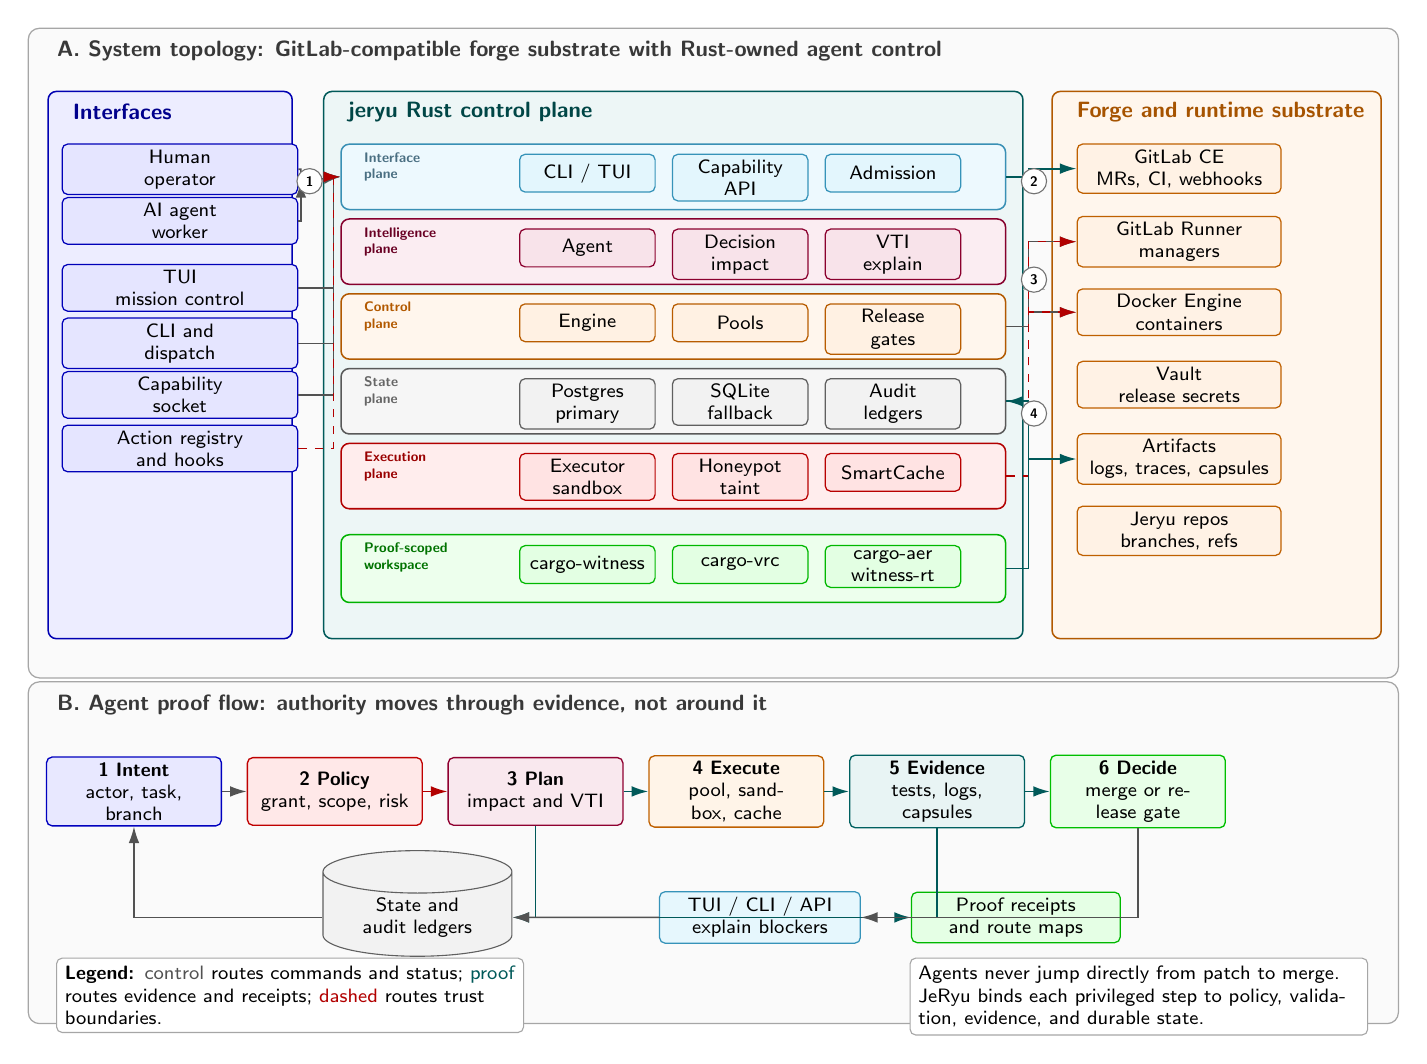
\begin{tikzpicture}[
    x=1cm,
    y=1cm,
    font=\sffamily\scriptsize,
    panel/.style={draw=black!35, fill=black!2, rounded corners=4pt, line width=0.45pt},
    title/.style={font=\sffamily\bfseries\footnotesize, text=black!78},
    lane/.style={draw=#1!70!black, fill=#1!7, rounded corners=3pt, line width=0.55pt},
    box/.style={draw=#1!72!black, fill=#1!11, rounded corners=2pt, line width=0.45pt,
        minimum height=0.48cm, align=center, text width=1.58cm, inner sep=2pt},
    widebox/.style={draw=#1!72!black, fill=#1!10, rounded corners=2pt, line width=0.45pt,
        minimum height=0.55cm, align=center, text width=2.85cm, inner sep=2pt},
    extbox/.style={draw=#1!75!black, fill=#1!10, rounded corners=2pt, line width=0.45pt,
        minimum height=0.56cm, align=center, text width=2.45cm, inner sep=2pt},
    datastore/.style={draw=#1!75!black, fill=#1!10, cylinder, shape border rotate=90,
        aspect=0.25, minimum height=0.62cm, minimum width=1.88cm, align=center,
        text width=1.55cm, inner sep=1.5pt},
    statebox/.style={draw=#1!75!black, fill=#1!10, rounded corners=2pt, line width=0.45pt,
        minimum height=0.48cm, align=center, text width=1.58cm, inner sep=2pt},
    plabel/.style={font=\sffamily\bfseries\tiny, align=left, text width=1.55cm},
    flowstep/.style={draw=#1!75!black, fill=#1!9, rounded corners=2pt, line width=0.48pt,
        minimum width=2.22cm, minimum height=0.86cm, align=center, text width=2.02cm, inner sep=2pt},
    control/.style={-{Latex[length=2.1mm,width=1.35mm]}, line width=0.55pt, draw=black!68},
    proof/.style={-{Latex[length=2.1mm,width=1.35mm]}, line width=0.65pt, draw=teal!70!black},
    guard/.style={-{Latex[length=2.1mm,width=1.35mm]}, line width=0.58pt, draw=red!70!black, dashed},
    rail/.style={line width=0.4pt, draw=black!28},
    badge/.style={circle, draw=black!55, fill=white, inner sep=0.8pt,
        font=\sffamily\bfseries\tiny, minimum size=0.32cm}
]

% ------------------------------------------------------------------
% Panel A: static system topology.  All arrows use rails so they do not
% cross boxes; this is intentionally closer to a C4 container diagram
% than a module dependency graph.
% ------------------------------------------------------------------
\node[panel, minimum width=17.4cm, minimum height=8.25cm, anchor=north west] (top) at (0,8.25) {};
\node[title, anchor=west] at (0.25,7.95) {A. System topology: GitLab-compatible forge substrate with Rust-owned agent control};

\node[lane=blue, minimum width=3.10cm, minimum height=6.95cm, anchor=north west] (surfaces) at (0.25,7.45) {};
\node[title, text=blue!55!black, anchor=west] at (0.45,7.18) {Interfaces};
\node[widebox=blue, anchor=north west] (human) at (0.43,6.78) {Human\\operator};
\node[widebox=blue, anchor=north west] (aiagent) at (0.43,6.10) {AI agent\\worker};
\node[widebox=blue, anchor=north west] (tui) at (0.43,5.25) {TUI\\mission control};
\node[widebox=blue, anchor=north west] (cli) at (0.43,4.57) {CLI and\\dispatch};
\node[widebox=blue, anchor=north west] (capability) at (0.43,3.89) {Capability\\socket};
\node[widebox=blue, anchor=north west] (actions) at (0.43,3.21) {Action registry\\and hooks};

\node[lane=teal, minimum width=8.88cm, minimum height=6.95cm, anchor=north west] (jeryu) at (3.75,7.45) {};
\node[title, text=teal!55!black, anchor=west] at (3.95,7.18) {jeryu Rust control plane};

\node[lane=cyan, minimum width=8.44cm, minimum height=0.83cm, anchor=north west] (interfaceplane) at (3.97,6.78) {};
\node[plabel, text=cyan!45!black, anchor=west] at (4.15,6.48) {Interface\\plane};
\node[box=cyan, anchor=north west] at (6.24,6.65) {CLI / TUI};
\node[box=cyan, anchor=north west] at (8.18,6.65) {Capability API};
\node[box=cyan, anchor=north west] at (10.12,6.65) {Admission};

\node[lane=purple, minimum width=8.44cm, minimum height=0.83cm, anchor=north west] (intelplane) at (3.97,5.83) {};
\node[plabel, text=purple!55!black, anchor=west] at (4.15,5.53) {Intelligence\\plane};
\node[box=purple, anchor=north west] at (6.24,5.70) {Agent};
\node[box=purple, anchor=north west] at (8.18,5.70) {Decision\\impact};
\node[box=purple, anchor=north west] at (10.12,5.70) {VTI\\explain};

\node[lane=orange, minimum width=8.44cm, minimum height=0.83cm, anchor=north west] (controlplane) at (3.97,4.88) {};
\node[plabel, text=orange!70!black, anchor=west] at (4.15,4.58) {Control\\plane};
\node[box=orange, anchor=north west] at (6.24,4.75) {Engine};
\node[box=orange, anchor=north west] at (8.18,4.75) {Pools};
\node[box=orange, anchor=north west] at (10.12,4.75) {Release\\gates};

\node[lane=gray, minimum width=8.44cm, minimum height=0.83cm, anchor=north west] (stateplane) at (3.97,3.93) {};
\node[plabel, text=black!60, anchor=west] at (4.15,3.63) {State\\plane};
\node[statebox=gray, anchor=north west] (postgres) at (6.24,3.80) {Postgres\\primary};
\node[statebox=gray, anchor=north west] (sqlite) at (8.18,3.80) {SQLite\\fallback};
\node[statebox=gray, anchor=north west] at (10.12,3.80) {Audit\\ledgers};

\node[lane=red, minimum width=8.44cm, minimum height=0.83cm, anchor=north west] (execplane) at (3.97,2.98) {};
\node[plabel, text=red!60!black, anchor=west] at (4.15,2.68) {Execution\\plane};
\node[box=red, anchor=north west] at (6.24,2.85) {Executor\\sandbox};
\node[box=red, anchor=north west] at (8.18,2.85) {Honeypot\\taint};
\node[box=red, anchor=north west] at (10.12,2.85) {SmartCache};

\node[lane=green, minimum width=8.44cm, minimum height=0.86cm, anchor=north west] (proofcrates) at (3.97,1.82) {};
\node[plabel, text=green!45!black, anchor=west] at (4.15,1.52) {Proof-scoped\\workspace};
\node[box=green, anchor=north west] at (6.24,1.68) {cargo-witness};
\node[box=green, anchor=north west] at (8.18,1.68) {cargo-vrc};
\node[box=green, anchor=north west] at (10.12,1.68) {cargo-aer\\witness-rt};

\node[lane=orange, minimum width=4.18cm, minimum height=6.95cm, anchor=north west] (substrate) at (13.00,7.45) {};
\node[title, text=orange!65!black, anchor=west] at (13.20,7.18) {Forge and runtime substrate};
\node[extbox=orange, anchor=north west] (gitlab) at (13.32,6.78) {GitLab CE\\MRs, CI, webhooks};
\node[extbox=orange, anchor=north west] (runner) at (13.32,5.86) {GitLab Runner\\managers};
\node[extbox=orange, anchor=north west] (docker) at (13.32,4.94) {Docker Engine\\containers};
\node[extbox=orange, anchor=north west] (vault) at (13.32,4.02) {Vault\\release secrets};
\node[extbox=orange, anchor=north west] (artifacts) at (13.32,3.10) {Artifacts\\logs, traces, capsules};
\node[extbox=orange, anchor=north west] (repos) at (13.32,2.18) {Jeryu repos\\branches, refs};

% Topology rails.
\draw[rail] (3.47,6.30) -- (3.72,6.30);
\draw[rail] (12.64,4.93) -- (12.92,4.93);
\draw[control] (human.east) -| (3.47,6.30) -- (interfaceplane.west);
\draw[control] (aiagent.east) -| (3.47,6.30);
\draw[control] (tui.east) -- ++(0.45,0) |- (interfaceplane.west);
\draw[control] (cli.east) -- ++(0.45,0) |- (interfaceplane.west);
\draw[control] (capability.east) -- ++(0.45,0) |- (interfaceplane.west);
\draw[guard] (actions.east) -- ++(0.45,0) |- (interfaceplane.west);

\draw[proof] (interfaceplane.east) -- ++(0.28,0) |- (gitlab.west);
\draw[control] (controlplane.east) -- ++(0.28,0) |- (runner.west);
\draw[control] (controlplane.east) -- ++(0.28,0) |- (docker.west);
\draw[guard] (execplane.east) -- ++(0.28,0) |- (runner.west);
\draw[guard] (execplane.east) -- ++(0.28,0) |- (docker.west);
\draw[proof] (stateplane.east) -- ++(0.28,0) |- (artifacts.west);
\draw[proof] (proofcrates.east) -- ++(0.28,0) |- (stateplane.east);

\node[badge] at (3.58,6.30) {1};
\node[badge] at (12.78,6.30) {2};
\node[badge] at (12.78,5.05) {3};
\node[badge] at (12.78,3.35) {4};

% ------------------------------------------------------------------
% Panel B: dynamic proof flow.  The row is intentionally linear; the
% feedback paths return on a lower rail instead of crossing the steps.
% ------------------------------------------------------------------
\node[panel, minimum width=17.4cm, minimum height=4.34cm, anchor=north west] (bottom) at (0, -0.05) {};
\node[title, anchor=west] at (0.25,-0.35) {B. Agent proof flow: authority moves through evidence, not around it};

\node[flowstep=blue] (f1) at (1.35,-1.45) {\textbf{1 Intent}\\actor, task, branch};
\node[flowstep=red] (f2) at (3.90,-1.45) {\textbf{2 Policy}\\grant, scope, risk};
\node[flowstep=purple] (f3) at (6.45,-1.45) {\textbf{3 Plan}\\impact and VTI};
\node[flowstep=orange] (f4) at (9.00,-1.45) {\textbf{4 Execute}\\pool, sandbox, cache};
\node[flowstep=teal] (f5) at (11.55,-1.45) {\textbf{5 Evidence}\\tests, logs, capsules};
\node[flowstep=green] (f6) at (14.10,-1.45) {\textbf{6 Decide}\\merge or release gate};

\draw[control] (f1.east) -- (f2.west);
\draw[guard] (f2.east) -- (f3.west);
\draw[proof] (f3.east) -- (f4.west);
\draw[proof] (f4.east) -- (f5.west);
\draw[proof] (f5.east) -- (f6.west);

\node[datastore=gray, minimum width=2.40cm, text width=2.05cm] (ledger) at (4.95,-3.05) {State and\\audit ledgers};
\node[widebox=cyan, minimum width=2.55cm, text width=2.25cm] (feedback) at (9.30,-3.05) {TUI / CLI / API\\explain blockers};
\node[widebox=green, minimum width=2.65cm, text width=2.35cm] (receipts) at (12.55,-3.05) {Proof receipts\\and route maps};

\draw[proof] (f5.south) |- (ledger.east);
\draw[proof] (f3.south) |- (receipts.west);
\draw[control] (f6.south) |- (feedback.east);
\draw[control] (feedback.west) -- (ledger.east);
\draw[control] (ledger.west) -| (f1.south);

\node[draw=black!35, fill=white, rounded corners=2pt, align=left, text width=5.72cm,
    anchor=north west, inner sep=3pt] at (0.36,-3.56) {
    \textbf{Legend:}
    \textcolor{black!68}{control} routes commands and status;
    \textcolor{teal!70!black}{proof} routes evidence and receipts;
    \textcolor{red!70!black}{dashed} routes trust boundaries.
};

\node[draw=black!35, fill=white, rounded corners=2pt, align=left, text width=5.60cm,
    anchor=north west, inner sep=3pt] at (11.20,-3.56) {
    Agents never jump directly from patch to merge. JeRyu binds each privileged step to policy, validation, evidence, and durable state.
};

\end{tikzpicture}
\end{adjustbox}
\caption{JeRyu architecture as described in \texttt{docs/ARCHITECTURE.md}. GitLab remains the forge and CI substrate, while the Rust \texttt{jeryu} control plane owns agent authority, runner policy, validation planning, cache trust, evidence capture, merge gates, and release gates.}
\label{fig:architecture-appendix}
\end{figure*}

\clearpage
\onecolumn
\raggedbottom
\section{Agent API and Control Surface Reference}
\label{app:agent-api}

\newcommand{\apicmd}[1]{\texttt{\footnotesize #1}}
\newcommand{\apicode}[1]{\texttt{\footnotesize #1}}
\newcommand{\apitabletitle}[1]{\par\medskip\begin{center}\small\textsc{#1}\end{center}\vspace{-0.7em}}
\setlength{\tabcolsep}{3pt}
\renewcommand{\arraystretch}{1.12}

This appendix is the agent-facing contract for the V3.01 repository. It is grounded in the active \apicode{jeryu} binary, the Unix-socket capability API, the native MCP server, the engine HTTP routes, the GitLab Runner custom executor protocol, the Git server admission hook, and the canonical action registry. The MCP surface is not a parallel authority system: it is a standards-compatible transport for the same policy, evidence, grant, and merge/release checks exposed through the existing capability model.

Git compatibility is handled through \apicode{jeryu git <args>} passthrough plus the native \apicode{jeryu save}, \apicode{jeryu sync}, and \apicode{jeryu undo} wrappers. The removed \apicode{ship} command and the old repo-mirror entrypoints no longer own a separate jeryu-git control plane.

\subsection{Surface Map}

\apitabletitle{Agent-Relevant API Surfaces}
\begin{center}
\small
\begin{tabular}{@{}p{0.15\linewidth}p{0.13\linewidth}p{0.20\linewidth}p{0.16\linewidth}p{0.24\linewidth}@{}}
\toprule
\textbf{Surface} & \textbf{Transport} & \textbf{Primary Consumer} & \textbf{Auth/Gate} & \textbf{Use}\\
\midrule
CLI & process invocation & humans, local agents, scripts & local process authority, GitLab PAT where needed & lifecycle, tests, release, pools, evidence, host operations\\
TUI & terminal UI & human supervisors, screen-reading agents & local process authority & operational state, actions, logs, proof stack\\
Capability API & Unix domain socket JSON & supervised local agents & protocol envelope, nonce, optional grant proof & typed agent intents and action discovery\\
MCP server & stdio JSON-RPC; loopback Streamable HTTP & MCP-compatible local agents & MCP lifecycle plus capability policy & standard tool discovery and calls over the same grant/evidence gates\\
HTTP engine & HTTP & GitLab webhooks, local health checks & webhook token for \apicode{/hooks} & reconciliation, cache summary, webhooks\\
Server hook & stdin/stdout process hook & Git server / GitLab hook & admission ledger, optional enforce mode & pre-receive branch/ref policy\\
Custom executor & GitLab Runner protocol & runner managers & runner invocation contract & sandbox, cache, witness, failure capsule capture\\
Action registry & static JSON contract & CLI, TUI, capability clients & canonical risk/grant metadata & discover actions and required grants\\
\bottomrule
\end{tabular}
\end{center}

\begin{lstlisting}[style=api,language=bash,caption={Agent discovery and status entrypoints}]
jeryu action list --json
jeryu status
jeryu next --project-id 2 --ref-name main
jeryu explain-blocker job 14445
jeryu capability serve /tmp/jeryu-capability.sock
jeryu mcp serve
jeryu mcp serve-http
jeryu mcp tools --json
\end{lstlisting}

\clearpage
\subsection{CLI Command Catalog}

All command names are kebab-case at the shell. Defaults below match the current Clap definitions.

\apitabletitle{Lifecycle, TUI, Status, and Global Action Commands}
\begin{center}
\small
\begin{tabular}{@{}p{0.28\linewidth}p{0.13\linewidth}p{0.53\linewidth}@{}}
\toprule
\textbf{Command} & \textbf{Mode} & \textbf{Purpose}\\
\midrule
\apicmd{jeryu init} & mutating & Bootstrap GitLab, state DB, runners, secrets, compose files, and smoke setup.\\
\apicmd{jeryu bootstrap} & mutating & Hidden alias for \apicode{init}.\\
\apicmd{jeryu serve} & daemon & Start Docker/GitLab orchestration, hook install, cache supervisor, runner warmup, engine, and background workers.\\
\apicmd{jeryu down} & mutating & Drain runner managers and stop the GitLab stack.\\
\apicmd{jeryu status} & read & Show GitLab, Vault, pools, managed containers, jobs, release, and secret state.\\
\apicmd{jeryu git <args>} & mixed & Pass through to the system Git binary and preserve the hook-driven jeryu-git path.\\
\apicmd{jeryu save|sync|undo} & mixed & Convenience wrappers for add/commit, rebase+push, and soft reset.\\
\apicmd{jeryu tui [--once]} & UI/read & Launch the Ratatui dashboard or render one smoke frame.\\
\apicmd{jeryu tui --capture --tab <tab> --output <png>} & read/artifact & Deterministic Ratatui PNG capture. Tabs: mission, release, jobs, agents, tests, pools, cache, evidence, secrets.\\
\apicmd{jeryu tui --screenshot --tab <tab> --screenshot-hold-ms <ms>} & read/session & Hold a real terminal render for external screenshot tooling.\\
\apicmd{jeryu progress --project-id 2 --ref-name main [--json]} & read & Show lane-aware CI and release progress.\\
\apicmd{jeryu next --project-id 2 --ref-name main} & read & Print the highest-priority next action for a branch.\\
\apicmd{jeryu explain-blocker <job|release|merge> <id>} & read & Explain why an entity is blocked using DB/GitLab evidence.\\
\apicmd{jeryu action list [--json]} & read & Emit the canonical action registry for humans or agents.\\
\bottomrule
\end{tabular}
\end{center}

\clearpage
\apitabletitle{Pool, Job, Pipeline, Cache, and Host Commands}
\begin{center}
\small
\begin{tabular}{@{}p{0.32\linewidth}p{0.13\linewidth}p{0.51\linewidth}@{}}
\toprule
\textbf{Command} & \textbf{Mode} & \textbf{Purpose}\\
\midrule
\apicmd{jeryu pool list} & read & List pools, manager counts, paused state, executor, and runner id.\\
\apicmd{jeryu pool scale <name> <count>} & mutating & Scale a pool to an exact manager count.\\
\apicmd{jeryu pool pause|resume <name>} & mutating & Pause or resume runner intake.\\
\apicmd{jeryu pool drain <name>} & mutating & Pause, wait, and stop managers.\\
\apicmd{jeryu pool delete <name>} & mutating & Drain, delete DB record, and unregister runner.\\
\apicmd{jeryu pool rotate-token <name>} & mutating & Reset GitLab runner token and update manager config.\\
\apicmd{jeryu job list <project> [--status running,pending]} & read & List GitLab jobs by scope.\\
\apicmd{jeryu job trace <project> <job>} & read & Print GitLab job trace.\\
\apicmd{jeryu job play|cancel|retry <project> <job>} & mutating & Start manual jobs, cancel jobs, or retry failed jobs.\\
\apicmd{jeryu job explain <project> <job>} & read & Print latest structured failure capsule and retry advice.\\
\apicmd{jeryu job clear} & mutating & Clear local job and pipeline history.\\
\apicmd{jeryu pipeline explain|doctor|jobs <pipeline> [--project-id 2] [--json]} & read & Inspect release eligibility, health, and job timing.\\
\apicmd{jeryu pipeline jobs <pipeline> --ingest} & mutating & Store current job timing rows.\\
\apicmd{jeryu pipeline ingest|cancel <pipeline> [--project-id 2]} & mutating & Persist timings or cancel a pipeline.\\
\apicmd{jeryu pipeline bottlenecks [--limit 25] [--json]} & read & Report historical slow jobs from local timing ledger.\\
\apicmd{jeryu cache enable} & mutating & Configure Docker for SmartCache registry mirror.\\
\apicmd{jeryu cache doctor|status [--json]} & read & Check proxy/registry/cache state and metrics.\\
\apicmd{jeryu cache gc [--dry-run] [--json] [--older-than <age>] [--max-cache-gb <gb>]} & mutating & Garbage-collect manager caches and cache state.\\
\apicmd{jeryu logs <manager-id> [-n 50]} & read & Tail manager container logs.\\
\apicmd{jeryu host storage-audit|doctor [--json]} & read & Audit storage and host health.\\
\apicmd{jeryu host reclaim --mode <mode> (--plan|--apply)} & mutating & Run planned or applied reclaim.\\
\bottomrule
\end{tabular}
\end{center}

\clearpage
\apitabletitle{Agent, Jeryu, Test/VTI, Release, Secret, and Repo Commands}
\begin{center}
\small
\begin{tabular}{@{}p{0.33\linewidth}p{0.13\linewidth}p{0.50\linewidth}@{}}
\toprule
\textbf{Command} & \textbf{Mode} & \textbf{Purpose}\\
\midrule
\apicmd{jeryu agent spawn <project> --task <text>} & mutating & Create an autonomous task branch/MR/issue workflow.\\
\apicmd{jeryu agent list <project>} & read & List active agent MRs/issues.\\
\apicmd{jeryu agent merge <project> <mr> [--trust-tier trusted]} & mutating & Request merge through the risk gate.\\
\apicmd{jeryu test run --command <cmd> [--force]} & mutating & Run a command through an ephemeral GitLab CI pipeline.\\
\apicmd{jeryu test plan --command <cmd>} & read & Preview inferred image, tags, timeout, and runner class.\\
\apicmd{jeryu test batch --command <cmd>... [--max-parallel 3]} & mutating & Launch several validation pipelines concurrently.\\
\apicmd{jeryu test results|failed|retry <pipeline>} & mixed & Inspect or retry pipeline test jobs.\\
\apicmd{jeryu test impact --base <sha> --head <sha> [--json]} & read & Determine CI jobs and release gates needed for a diff.\\
\apicmd{jeryu test select [emit flags]} & read/artifact & Compute internal VTI plan and optionally emit GitLab YAML, JSON plan, and VTI receipt.\\
\apicmd{jeryu test explain-plan <plan.json>} & read & Explain a serialized VTI plan.\\
\apicmd{jeryu test select-external --workspace <root>} & read/artifact & Use external \apicode{.jeryu/testmap.toml}.\\
\apicmd{jeryu test audit|learn} & read & Compare VTI selections with oracle results and suggest rule changes.\\
\apicmd{jeryu test cache-status --base <sha> --head <sha> [--json]} & read & Show test-command cache state for the current source state.\\
\apicmd{jeryu release status|watch|reconcile} & mixed & Read or reconcile release attempts.\\
\apicmd{jeryu release promote-prod [--version <v>]} & mutating & Trigger approved production promotion after canary gates.\\
\apicmd{jeryu release preflight|doctor [--json]} & read & Check blockers, infrastructure, and release readiness.\\
\apicmd{jeryu secrets <subcommand>} & mixed & Manage Vault-backed release lifecycle: init, status, rotate, finalize, report, recover.\\
\apicmd{jeryu repo render-agent-index [--check]} & artifact/check & Generate or verify machine-readable agent routing index.\\
\apicmd{jeryu repo audit-agent-surface [--json]} & read & Audit routing docs, generated index, and agent surface freshness.\\
\bottomrule
\end{tabular}
\end{center}

\subsection{Exact CLI Grammar}

The following grammar is generated from the active Clap definitions in \apicode{src/cli.rs}. It includes hidden protocol calls because those are part of the agent and runner contract even though they are not intended for direct human operation.

\begin{lstlisting}[style=api,language=bash,caption={Exhaustive jeryu command forms}]
jeryu init
jeryu bootstrap
jeryu serve
jeryu down
jeryu status
jeryu logs <manager-id> [-n <lines>]
jeryu progress [--project-id <id>] [--ref-name <ref>] [--json]
jeryu next [--project-id <id>] [--ref-name <ref>]
jeryu explain-blocker <job|release|merge> <id>

jeryu tui [--once]
jeryu tui --capture [--tab <tab>] [--output <path>] [--width <cols>] [--height <rows>]
jeryu tui --screenshot [--tab <tab>] [--width <cols>] [--height <rows>] [--screenshot-hold-ms <ms>]

jeryu action list [--json]

jeryu pool list
jeryu pool scale <name> <count>
jeryu pool pause <name>
jeryu pool resume <name>
jeryu pool drain <name>
jeryu pool delete <name>
jeryu pool rotate-token <name>

jeryu job list <project-id> [--status <csv>]
jeryu job trace <project-id> <job-id>
jeryu job play <project-id> <job-id>
jeryu job cancel <project-id> <job-id>
jeryu job retry <project-id> <job-id>
jeryu job explain <project-id> <job-id>
jeryu job clear

jeryu pipeline explain [--project-id <id>] <pipeline-id> [--json]
jeryu pipeline doctor [--project-id <id>] <pipeline-id> [--json]
jeryu pipeline jobs [--project-id <id>] <pipeline-id> [--ingest] [--json]
jeryu pipeline ingest [--project-id <id>] <pipeline-id>
jeryu pipeline cancel [--project-id <id>] <pipeline-id>
jeryu pipeline bottlenecks [--project-id <id>] [--ref-name <ref>] [--limit <n>] [--json]

jeryu cache enable
jeryu cache doctor
jeryu cache status [--json]
jeryu cache gc [--dry-run] [--json] [--keep-active-managers[=true|false]] [--older-than <age>] [--max-cache-gb <gb>]

jeryu agent spawn <project-id> --task <text>
jeryu agent list <project-id>
jeryu agent merge <project-id> <mr-iid> [--trust-tier <tier>]

jeryu test run --command <cmd> [--project-id <id>] [--image <image>] [--tags <csv>] [--timeout <sec>] [--force]
jeryu test plan --command <cmd> [--project-id <id>] [--image <image>] [--tags <csv>] [--timeout <sec>]
jeryu test batch --command <cmd>... [--project-id <id>] [--image <image>] [--tags <csv>] [--timeout <sec>] [--max-parallel <n>] [--force]
jeryu test results <pipeline-id> [--project-id <id>]
jeryu test retry <pipeline-id> <job-name> [--project-id <id>]
jeryu test failed <pipeline-id> [--project-id <id>]
jeryu test impact --base <ref> --head <ref> [--repo-root <path>] [--json]
jeryu test select [--base <ref>] [--head <ref>] [--repo-root <path>] [--explain] [--json] [--emit-gitlab <path>] [--emit-plan <path>] [--emit-receipt <path>]
jeryu test explain-plan <plan-path>
jeryu test select-external [--base <ref>] [--head <ref>] --workspace <path> [--explain] [--json] [--emit-gitlab <path>] [--emit-plan <path>] [--emit-skipped <path>]
jeryu test audit --changed <csv> --all-tests <csv> [--failed <csv>] [--sha <sha>] [--json] [--workspace <path>]
jeryu test learn --changed <csv> --all-tests <csv> [--failed <csv>] [--sha <sha>] [--json] [--workspace <path>]
jeryu test cache-status [--base <ref>] [--head <ref>] [--json]

jeryu release status [--project-id <id>] [--ref-name <ref>] [--sha <sha>] [--limit <n>] [--json]
jeryu release watch [--project-id <id>] [--ref-name <ref>] [--sha <sha>] [--limit <n>] [--interval-secs <sec>] [--json]
jeryu release reconcile [--project-id <id>] [--ref-name <ref>] [--json]
jeryu release promote-prod [--project-id <id>] [--ref-name <ref>] [--version <version>]
jeryu release preflight [--ssh-host <host>] [--json]
jeryu release doctor [--version <version>] [--preflight[=true|false]] [--json]

jeryu secrets init
jeryu secrets status [--json]
jeryu secrets rotate [--repo <name>] --version <version> --target <target>
jeryu secrets finalize [--repo <name>] --version <version> --target <target>
jeryu secrets report [--repo <name>] --version <version>
jeryu secrets recover [--repo <name>] --version <version>

jeryu host storage-audit
jeryu host doctor [--json]
jeryu host reclaim --mode <mode> [--plan] [--apply]

jeryu repo render-agent-index [--check]
jeryu repo audit-agent-surface [--json]

jeryu exec config
jeryu exec prepare
jeryu exec run <script-path> <stage>
jeryu exec cleanup
jeryu server-hook pre-receive
jeryu capability serve <socket-path>
\end{lstlisting}

\clearpage
\subsection{Hidden Protocol Entrypoints}

\apitabletitle{Protocol Commands Not Intended for Direct Human Use}
\begin{center}
\small
\begin{tabular}{@{}p{0.29\linewidth}p{0.17\linewidth}p{0.49\linewidth}@{}}
\toprule
\textbf{Command} & \textbf{Caller} & \textbf{Contract}\\
\midrule
\apicmd{jeryu exec config} & GitLab Runner & Return custom executor driver configuration JSON.\\
\apicmd{jeryu exec prepare} & GitLab Runner & Prepare clone/sandbox/honeypot/cache context.\\
\apicmd{jeryu exec run <script> <stage>} & GitLab Runner & Run a build stage with cache brain, witnesses, tripwire handling, and capsule capture.\\
\apicmd{jeryu exec cleanup} & GitLab Runner & Clean executor state after job completion.\\
\apicmd{jeryu server-hook pre-receive} & Git server hook & Read ref updates from stdin and write admission decisions.\\
\apicmd{jeryu capability serve <socket>} & local supervisor & Start Unix-socket JSON capability API.\\
\bottomrule
\end{tabular}
\end{center}

\subsection{Capability Socket Protocol}

The capability API is a local Unix domain socket service. It accepts either a  tagged \apicode{AgentIntent} JSON document or the V3.01 \apicode{AgentActionRequest} envelope. New agents should use the envelope. The server also accepts an optional 4-byte big-endian length prefix before the JSON body. Responses use \apicode{CapabilityResponse}.

\begin{lstlisting}[style=api,language=rust,caption={V3.01 capability envelope}]
struct AgentActionRequest {
  protocol_version: "v3.01",
  request_id: String,
  actor: String,
  nonce: String,
  expires_at: Option<Rfc3339DateTime>,
  project_id: Option<i64>,
  base_ref: Option<String>,
  base_sha: Option<String>,
  idempotency_key: Option<String>,
  budget: Option<ActionBudget>,
  grant: Option<CapabilityGrantProof>,
  intent: AgentIntent
}

struct CapabilityResponse {
  success: bool,
  message: String,
  data: Option<JsonValue>
}
\end{lstlisting}

\begin{lstlisting}[style=api,language=json,caption={Envelope example: request a system snapshot}]
{
  "protocol_version": "v3.01",
  "request_id": "req-20260427-0001",
  "actor": "agent.codex.local",
  "nonce": "7f096ab2-9e0d-4d80-9c4b-42fb56c6d62d",
  "expires_at": "2026-04-27T10:15:00Z",
  "idempotency_key": "snapshot-main-001",
  "intent": { "intent": "GetSystemSnapshot" }
}
\end{lstlisting}

\apitabletitle{Envelope Validation and Replay Rules}
\begin{center}
\small
\begin{tabular}{@{}p{0.22\linewidth}p{0.72\linewidth}@{}}
\toprule
\textbf{Field/Rule} & \textbf{Behavior}\\
\midrule
\apicode{protocol\_version} & Must equal \apicode{v3.01}; other versions are rejected.\\
\apicode{request\_id} and \apicode{actor} & Required for enveloped requests and logged as request context.\\
\apicode{nonce} & Required and cached per actor; duplicate actor/nonce pairs are rejected as replay.\\
\apicode{expires\_at} & Optional RFC3339 timestamp; expired requests are rejected.\\
\apicode{budget} & Optional caller-declared time/branch/pipeline limits.\\
\apicode{grant} & Optional proof payload. Current code validates envelope shape and records grants for successful branch-writing intents; signed grant enforcement remains future hardening.\\
Legacy requests & Accepted for compatibility, tagged as \apicode{-capability-client}.\\
\bottomrule
\end{tabular}
\end{center}

\subsection{Capability Intents}

\apitabletitle{Capability Intents and Effects}
\begin{center}
\small
\begin{tabular}{@{}p{0.18\linewidth}p{0.15\linewidth}p{0.22\linewidth}p{0.41\linewidth}@{}}
\toprule
\textbf{Intent} & \textbf{Risk} & \textbf{Inputs} & \textbf{Result}\\
\midrule
\apicode{FetchCapsule} & read & \apicode{job\_id} & Return latest DB failure capsule for a job, or a structured miss.\\
\apicode{RunTests} & CI execution & \apicode{project\_id}, \apicode{target\_ref}, \apicode{test\_scope} & Create ephemeral branch, write dynamic CI YAML, trigger pipeline, record a 24-hour grant.\\
\apicode{ProposePatch} & git write & project, branch, base, commit message, file modifications, optional MR title & Create branch, commit changes, open MR, record grant bound to returned commit SHA.\\
\apicode{RacePatches} & git write / CI & project, base branch, commit message, hypotheses & Launch multiple hypothesis branches and pipelines; returns branches, pipeline ids, grant ids.\\
\apicode{RequestMerge} & production/merge & project, MR IID, source, target & Evaluate conservative merge gate proof using selector miss and cache taint checks.\\
\apicode{ExplainBlockers} & read & entity type and id & Explain blockers for job, release, or merge-like entity.\\
\apicode{GetSystemSnapshot} & read & none & Return pools, cache metrics, selector misses, recent failures, timestamp.\\
\apicode{ListAllowedActions} & read & none & Return capability-visible registry actions with risk/grant metadata.\\
\apicode{PlanValidation} & read & project, test ids, ref & Validate a proposed test list against recent selector misses.\\
\bottomrule
\end{tabular}
\end{center}

\begin{lstlisting}[style=api,language=json,caption={Legacy intent examples}]
{ "intent": "FetchCapsule", "payload": { "job_id": 14445 } }

{
  "intent": "RunTests",
  "payload": {
    "project_id": 2,
    "target_ref": "main",
    "test_scope": "unit"
  }
}

{
  "intent": "PlanValidation",
  "payload": {
    "project_id": 2,
    "ref_name": "main",
    "test_ids": ["unit:jeryu", "integration:job_tests"]
  }
}
\end{lstlisting}

\begin{lstlisting}[style=api,language=json,caption={ProposePatch payload shape}]
{
  "intent": "ProposePatch",
  "payload": {
    "project_id": 2,
    "branch_name": "agent/fix-cache-proof",
    "base_ref": "main",
    "commit_message": "fix: strengthen cache proof",
    "mr_title": "Agent patch: cache proof hardening",
    "modifications": [
      {
        "file_path": "src/cache_brain.rs",
        "content": "...complete replacement content..."
      }
    ]
  }
}
\end{lstlisting}

\subsection{HTTP Engine API}

\apitabletitle{Engine HTTP Routes}
\begin{center}
\small
\begin{tabular}{@{}p{0.10\linewidth}p{0.17\linewidth}p{0.22\linewidth}p{0.45\linewidth}@{}}
\toprule
\textbf{Method} & \textbf{Path} & \textbf{Auth} & \textbf{Behavior}\\
\midrule
GET & \apicode{/health} & none & Return \apicode{ok}.\\
POST & \apicode{/hooks} & \apicode{X-Gitlab-Token} matching \apicode{JERYU\_WEBHOOK\_SECRET} & Ingest GitLab job, pipeline, push, and MR webhooks.\\
GET & \apicode{/cache/summary} & none & Return cache health summary JSON.\\
\bottomrule
\end{tabular}
\end{center}

\begin{lstlisting}[style=api,language=bash,caption={HTTP route examples}]
curl http://127.0.0.1:9777/health

curl http://127.0.0.1:9777/cache/summary

curl -X POST http://127.0.0.1:9777/hooks \
  -H "X-Gitlab-Token: $JERYU_WEBHOOK_SECRET" \
  -H "X-Gitlab-Event: Push Hook" \
  --data-binary @push-hook.json
\end{lstlisting}

\apitabletitle{Webhook Event Behavior}
\begin{center}
\small
\begin{tabular}{@{}p{0.20\linewidth}p{0.74\linewidth}@{}}
\toprule
\textbf{Event} & \textbf{Behavior}\\
\midrule
Job Hook & Upsert job event, maybe auto-retry failures, scale up for pending/created work.\\
Pipeline Hook & Track pipeline state, launch canary on green main, update release/prod pipeline state.\\
Push Hook & Normalize ref, skip \apicode{jeryu-test-*}, cancel superseded pipelines, compute impact, persist VTI plan.\\
Merge Request Hook & Logged for observability; no privileged merge behavior.\\
Other & Logged as unhandled.\\
\bottomrule
\end{tabular}
\end{center}

\subsection{Action Registry Contract}

The action registry is the shared action catalog consumed by the TUI command palette, \apicode{jeryu action list}, and \apicode{ListAllowedActions}. Each entry exposes \apicode{id}, \apicode{label}, \apicode{key\_hint}, \apicode{risk\_tier}, \apicode{side\_effect\_class}, \apicode{required\_grant}, \apicode{dry\_run}, \apicode{surfaces}, and \apicode{description}.

\apitabletitle{Canonical Action Registry}
\begin{center}
\small
\begin{tabular}{@{}p{0.22\linewidth}p{0.13\linewidth}p{0.14\linewidth}p{0.16\linewidth}p{0.29\linewidth}@{}}
\toprule
\textbf{Action ID} & \textbf{Risk} & \textbf{Grant} & \textbf{Surfaces} & \textbf{Purpose}\\
\midrule
\apicode{open\_logs} & read-only & none & TUI & Open selected job logs.\\
\apicode{retry\_job} & low & agent task & CLI, TUI & Retry a failed or canceled job.\\
\apicode{delete\_record} & low & agent task & TUI & Remove local DB record.\\
\apicode{pause\_pool} & low & agent task & CLI, TUI & Pause or resume runner pool.\\
\apicode{explain\_blockers} & read-only & none & CLI, TUI, capability & Explain job/release/merge blockers.\\
\apicode{get\_system\_snapshot} & read-only & none & CLI, capability & Return system summary.\\
\apicode{propose\_patch} & high & agent task & CLI, TUI, capability & Create branch, patch, and MR.\\
\apicode{race\_patches} & high & agent task & CLI, capability & Launch competing hypotheses.\\
\apicode{request\_merge} & production & merge approval & CLI, TUI, capability & Request merge through gate.\\
\apicode{plan\_validation} & read-only & none & CLI, capability & Validate proposed test plan.\\
\apicode{run\_tests} & low & agent task & CLI, TUI, capability & Trigger targeted test pipeline.\\
\apicode{next\_action} & read-only & none & CLI, TUI & Print recommended next action.\\
\apicode{tab\_*} & read-only & none & TUI & Switch primary TUI tab from Mission through Secrets.\\
\apicode{toggle\_audit\_ledger} & read-only & none & TUI & Toggle Evidence tab view.\\
\apicode{quit} & read-only & none & TUI & Exit TUI.\\
\bottomrule
\end{tabular}
\end{center}

\begin{lstlisting}[style=api,language=json,caption={Action registry JSON excerpt}]
{
  "id": "request_merge",
  "label": "Request merge",
  "risk_tier": "production",
  "side_effect_class": "merge",
  "required_grant": "merge_approval",
  "dry_run": false,
  "surfaces": ["cli", "tui", "capability"],
  "description": "Merge an MR through the risk gate..."
}
\end{lstlisting}

\clearpage
\twocolumn
\flushbottom
\subsection{Native MCP Server}
\label{app:mcp-server}

V3.01 ships a native Model Context Protocol server for external coding agents that already speak MCP. The server is implemented as \apicode{src/mcp.rs} plus the \apicode{src/mcp/} module tree and is exposed through \apicode{jeryu mcp serve}, \apicode{jeryu mcp serve-http}, and \apicode{jeryu mcp tools --json}. Its purpose is deliberately narrow: translate MCP lifecycle and tool messages into the same typed \apicode{AgentIntent} execution path used by the Unix-socket capability API.

The important boundary is that MCP is a transport, not a privilege escalation path. A call to \apicode{jeryu.request\_merge} over MCP is evaluated by the same capability policy, grant metadata, durable evidence recording, GitLab client wrapper, and merge/release gate logic as the equivalent native capability request. Read-only tools remain read-only; branch-writing tools still create explicit branches and evidence; production-sensitive tools still require the same gate decisions.

\begin{table}[t]
\centering
\tiny
\caption{MCP server transports and lifecycle}
\begin{tabular}{@{}p{0.34\columnwidth}p{0.56\columnwidth}@{}}
\toprule
\textbf{Surface} & \textbf{Behavior}\\
\midrule
\apicode{stdio} & JSON-RPC line protocol for local agents launched as child processes by editors, terminals, or agent runtimes.\\
\apicode{HTTP} & Streamable HTTP endpoint at \apicode{/mcp}, bound to loopback by default through \apicode{settings.mcp.bind}.\\
\apicode{initialize} & Negotiates protocol version \apicode{2025-11-25}, returns \apicode{serverInfo}, and advertises tool support.\\
\shortstack[l]{\apicode{notifications/}\\\apicode{initialized}} & Marks the session initialized and records client attribution for later capability context.\\
\apicode{ping} & Lightweight liveness check for clients that keep long-running sessions.\\
\apicode{tools/list} & Returns the canonical tool manifest derived from the action registry.\\
\apicode{tools/call} & Parses tool arguments, builds an \apicode{AgentIntent}, executes it through capability policy, and returns MCP content plus structured result data.\\
\bottomrule
\end{tabular}
\end{table}

\begin{table}[t]
\centering
\tiny
\caption{MCP tool surface}
\begin{tabular}{@{}p{0.45\columnwidth}p{0.45\columnwidth}@{}}
\toprule
\textbf{Tool} & \textbf{Function}\\
\midrule
\shortstack[l]{\apicode{jeryu.get\_system}\\\apicode{\_snapshot}} & Read current operational state for jobs, pools, release, and evidence.\\
\shortstack[l]{\apicode{jeryu.explain}\\\apicode{\_blockers}} & Explain why a job, release, or merge is blocked.\\
\shortstack[l]{\apicode{jeryu.plan}\\\apicode{\_validation}} & Produce a VTI-backed validation plan for selected tests and refs.\\
\shortstack[l]{\apicode{jeryu.fetch}\\\apicode{\_capsule}} & Fetch structured failure capsule data for a job.\\
\shortstack[l]{\apicode{jeryu.run}\\\apicode{\_tests}} & Create an ephemeral validation branch and trigger CI for a scoped test run.\\
\shortstack[l]{\apicode{jeryu.propose}\\\apicode{\_patch}} & Create a branch, apply file modifications, commit, and open a merge request.\\
\shortstack[l]{\apicode{jeryu.race}\\\apicode{\_patches}} & Launch multiple patch hypotheses while preserving branch-level evidence.\\
\shortstack[l]{\apicode{jeryu.request}\\\apicode{\_merge}} & Ask the merge gate to evaluate an MR against release and risk policy.\\
\bottomrule
\end{tabular}
\end{table}

Tool discovery is schema-bearing. Each MCP tool includes an \apicode{inputSchema}, an \apicode{outputSchema}, and MCP annotations such as \apicode{readOnlyHint}, \apicode{destructiveHint}, \apicode{idempotentHint}, and \apicode{openWorldHint}. These annotations are derived from the same action-risk vocabulary used by the CLI and TUI registry, so an agent does not need a separate policy document to know which tools are read-only, mutating, or production-sensitive.

The HTTP transport adds local-server hardening around the same core. It refuses non-loopback bind addresses at startup, rejects non-local \apicode{Origin} headers, returns \apicode{Mcp-Session-Id} on \apicode{initialize}, requires that session id on later requests, requires \apicode{MCP-Protocol-Version} after initialization, validates \apicode{Mcp-Method} and \apicode{Mcp-Name} against the JSON-RPC body, and supports \apicode{DELETE /mcp} for explicit session teardown. \apicode{GET /mcp} returns \apicode{405}; this implementation is a POST-oriented local control surface rather than an event-streaming API.

\begin{lstlisting}[style=api,language=json,caption={MCP tool call shape}]
{
  "jsonrpc": "2.0",
  "id": 7,
  "method": "tools/call",
  "params": {
    "name": "jeryu.explain_blockers",
    "arguments": {
      "entity_type": "merge",
      "entity_id": 42
    }
  }
}
\end{lstlisting}

The response shape is intentionally useful to both simple chat agents and structured orchestrators. MCP \apicode{content} carries a human-readable text summary, while \apicode{structuredContent} carries the native capability response with \apicode{success}, \apicode{message}, and optional data. When the underlying capability call fails, the server sets \apicode{isError} without hiding the structured policy result. This lets clients present a concise explanation to a human while still preserving machine-readable evidence for retries, escalation, or audit.


\bibliographystyle{IEEEtran}
\bibliography{references}
\end{document}
